\chapter{Data processing}
\label{ch:data_processing}

Events recorded by \hisparc electronics consist of the \pmt readouts (traces) and a trigger timestamp. Before events can be used in analysis observables have to be extracted. For the core and direction reconstructions the particle count and arrival time for each detector are used. These values can be derived from the traces and trigger timestamp using calibration values and configuration settings. The following sections will detail each step of the processing. Part of the processing is performed on the station PC because some observables provide insight into the proper working of the detectors and the calibration of the \pmts. Other observables which are determined using multiple events and those for which the algorithm is subject to change are determined offline at \nikhef.


\section{Online processing}
\label{sec:online}

% On the HiSPARC PC
% This data is sent to/stored in the datastore (Table 3.1 Fokkema);
% ext_timestamp, data_reduction, trigger_pattern, baseline, std_dev, n_peaks, pulseheights, integrals, traces, event_rate
When the \hisparc electronics trigger the detected signal traces and timing information is sent to the controlling PC. First the PC determines the absolute \gps timestamp for the event, as explained in \cref{sub:gps_timestamps}. The PC then analyses each trace individually to determine several event properties, these processes are described in the following sections.


\subsection{Trace baseline}

% Baseline can deviate from desired value
% Thresholds are based on absolute ADC count values
% How baseline is determined from trace
% Why it can fail, how often that happens
Even though the \adcs are calibrated the baselines can still shift away from the desired value and can fluctuate over time. Therefore, the baseline must be determined for each trace. There is a high probability that the pre-trigger window part of the event traces do not contain a significant signal and is therefore suitable for baseline determination. The rate of singles is low enough that the probability of a coincidental signal is less than \SI{0.1}{\percent}. Moreover, if there was a large signal in that window it would likely have been part of the trigger. Hence the first part of a trace is usually suitable for determining its baseline. An algorithm checks if the start of the trace is smooth enough to be used for the baseline. The algorithm compares each sample to the average value up to and including the previous sample. The difference must be less than the baseline-threshold, which is usually set to \SI{17}{\adc} or \SI{10}{\milli\volt}. Additionally, the difference between the current and previous samples must be less than twice this threshold. At least the first 50 samples (i.e. \SI{125}{\ns}) must satisfy the smoothness criteria, but more can be used. If that is the case then the average of those samples will be the baseline.

If the start of the trace is not smooth the baseline can not be determined and will be set to the error value \num{-999}. The algorithm has recently been updated to also attempt to find a baseline from the end of the trace if it does not succeed from the start. The udpated algorithm has not yet been retroactively applied to existing traces for which no good baseline was found. Once the baseline is known other properties can be determined, if the baseline can not be determined all other properties dependent on it are also set to \num{-999}. In a properly operating station the baseline determination hardly ever fails. The probability of a significant signal to prevent baseline determination, but not strong enough to be part of the trigger, within the first \SI{125}{\ns} is extremely low.

Deviations of the baseline to the desired value are represented in a histogram in the \hisparc \daq interface. If the baseline deviation is to large this affects the trigger thresholds because those assume the correct baseline.


\subsection{Signal strength}

% Pulse height and integral determination
% Requires good baseline
% integral definition
The pulse height is the value of the highest signal in the trace, relative to the baseline. With the baseline calibrated to \SI{200}{\adc} the highest possible pulse height is $4096 - 200 = \SI{3896}{\adc}$. For most stations this value is rarely attained, because most \pmts are unable to produce large enough signals, as discussed in \cref{sub:pmt_linearity}. For stations with new \pmts saturated signals occur multiple times per day. For each triggered event in a 2-detector station, using the default triggering, both detectors should have a pulse height at least equal to the low threshold, since that is the trigger condition. This may fluctuate due to fluctuations in the baseline, because the trigger thresholds are absolute thresholds, not relative to the actual baseline. In 4-detector stations the most common trigger is two high signals in two detectors, with no signals in the other two detectors. So in a 4-detector station events can have detectors with pulse heights less than the trigger thresholds.

The pulse integral is the integral of the area under the signals. However, only signals that are at least the baseline-threshold above the baseline are included. The threshold filters signal noise, reflections, and small peaks from the integral. The pulse integral more accurately represents the particle count in a detector, since it also acounts for signals which are separated in time. In \cref{fig:integral} the pulse height and integral are illustrated.

As soon as the \hisparc \daq starts data taking it will begin to accumulate the determined pulse heights and integrals in histograms. These histograms can be used to determine by eye if the \mpv is clearly visible and above the thresholds but not to high. If this is not the case the \pmts voltage need to be adjusted. About half an hour of data is needed to properly asses this.

\begin{figure}
    \centering
    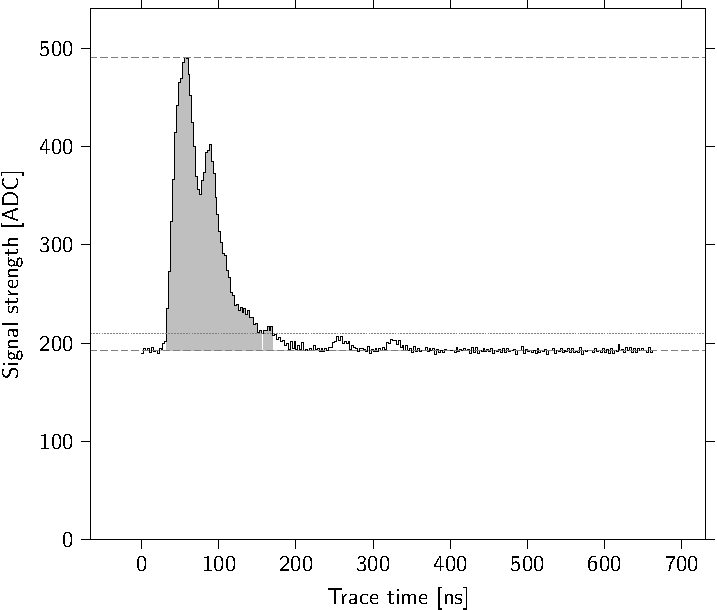
\includegraphics[width=0.7\linewidth]{plots/processing/integral}
    \caption{Illustrated definition of the pulse height and integral for a signal trace (solid line). The baseline (lower dashed line) was determined using the pre-trigger window of the trace (not shown). The pulse height is the space between the two dashed lines. The integral is indicated by the shaded area, only signals above the threshold (dotted line) count towards the integral.}
    \label{fig:integral}
\end{figure}


\subsection{Signal structure}

% Some other observables, number of peaks and standard deviation
Most traces contain only a single pulse. However, sometimes multiple particles pass through a detector within the short time window of the trigger, and separated enough to be distinguishable in the trace. In order to find events with multiple pulses the number of peaks in a trace is determined. The algorithm starts at the start of a trace and when the signal values rise more than the low trigger threshold, in this case relative to the baseline, a peak is counted. When a peak has reached its apex and then lowers again the maximum value is remembered, the trace values needs to drop at least the value of the threshold before a new peak can start. For the next peak the signal value needs to rise at least the threshold value again, above the new local minimum since the previous peak. This is illustrated in \cref{fig:n_peaks}.

\begin{figure}
    \centering
    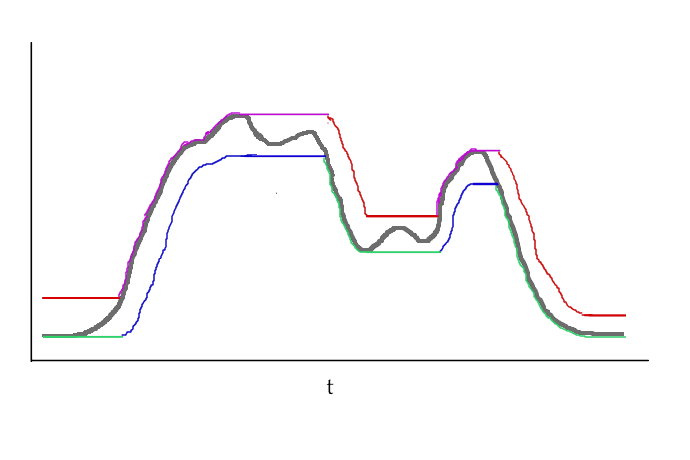
\includegraphics[width=0.7\linewidth]{plots/processing/n_peaks}
    \caption{Illustrated definition of the number of peaks. The shown trace (gray) has multiple bumps, but not all are actual peaks. The thresholds the signal needs to cross to be counted as peak (red), and the threshold is need to drop below before the next peak can start (blue) are shown. These thresholds follow the local minimum (green) and local maximum (purple). In this case two peaks are seen.}
    \label{fig:n_peaks}
\end{figure}

The number of peaks can be a good indication of light leaks, which result in many small peaks in traces. A single event with many peaks does not immediately indicate a light leak, however, if occurs very often for a detector that may be indicative. A histogram with the number of peaks is therefore also shown in the \hisparc \daq.

The ratio between the pulse height and integral also provides structure information. If the pulse integral is higher than expected for a given pulse height, then the trace probably contains multiple peaks, or the \adcs are saturated limiting the maximum pulse height.

As a measure of the stability of the trace around the baseline the standard deviation of the same part of the trace that was used for the baseline is calculated. This can be used as an indicator for the misalignment of the \adcs.


\subsection{Data reduction}

% Data reduction to reduce load on uploading and datastore
% Unfortunately introduced data loss
% Partly saved by sending unreduced trace every so often
Most events contain only two pulses in two detectors. These pulses are often very correlated in time (at least within the \SI{1.5}{\micro\second} trigger window) and normal small pulses are \SIrange{30}{100}{\ns} long. The rest of the trace is usually empty, and contains no valuable data. For each event the part containing all significant pulses is determined. The algorithm looks from the start and end of the traces up to the point that any of the detectors has a pulse, which is defined as a signal more than the baseline-threshold above the determined baselines. The empty parts of the traces will be cut away, except for a padding of \num{26} samples around the cuts on both sides, these extra samples allow verification of the baseline in the offline analysis. On average (median) this leads to traces with \SI{150}{\ns} (i.e. 60 samples) length, including [or excluding?] the padding. The default trace length (pre-trigger, trigger, post-trigger windows) is \SI{6}{\micro\second} (i.e. 2400 samples). Overall \SI{2.5}{\percent} of the measured data is kept. This greatly reduces the size of data to be transferred to the datastore and to be analysed offline.  Unfortunately a bug in the \daq software caused this padding to be missing for many events, preventing offline baseline reconstruction. However, approximately every \SI{40}{\minute} the full traces of an event are kept to provide more information for offline analysis. This also allows for a quality check of the baselines.

\begin{figure}
    \centering
    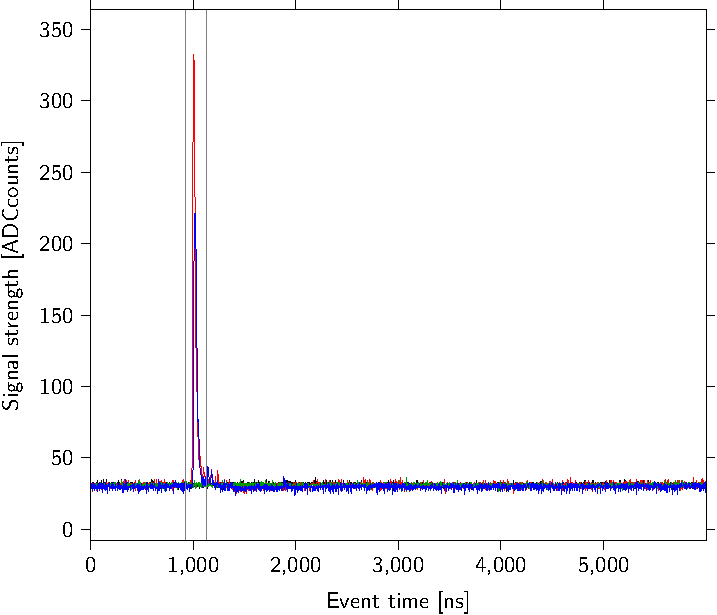
\includegraphics[width=0.4\textwidth]{plots/processing/raw_trace_region_reduced}
    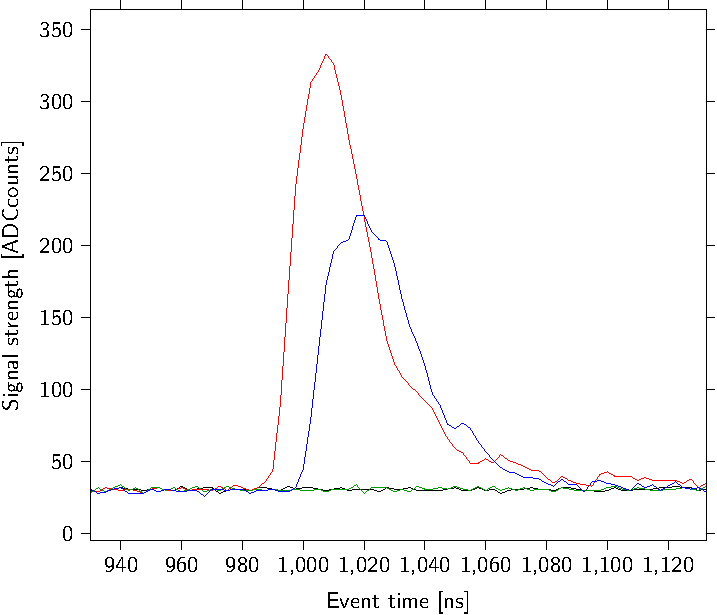
\includegraphics[width=0.4\textwidth]{plots/processing/reduced_traces}
    \caption{The original raw traces of a single event (left) and the reduced traces (right) are shown. The vertical lines indicate the region which is to be kept. Outside that region none of the trace samples are over the baseline-threshold of \SI{17}{\adc} above the baseline.}
    \label{fig:data_reduction}
\end{figure}

% Script to determine some values, to be determined for larger dataset:
% lengths = [zlib.decompress(s.blobs[i]).count(',') for i in range(0, s.blobs.nrows, 4)]
% median(lengths)
% mean([l for l in lengths if l != 2400])
% len([l for l in lengths if l == 2400])


\subsection{Mean filter}
\label{ssec:mean_filter}

% Another destructive process
% May prevent trigger time reconstruction
% Is useful to smoothen trace and perhaps get more realistic values
% Does not perfectly solve different baselines and gains for the channels..
During the setup of a station the separate \adcs for each channel in the \hisparc electronics are aligned, however, this alignment is not perfect and can change over time. Typically a saw-tooth pattern can be observed in the measured traces. The amplitude of the saw-tooth can be different at different signal levels, because both the offset and gain may be different. This can be filtered out by averaging the signal. This is a multi-step process. First the trace is split into the even and odd parts (positive and negative clock) which are smoothed separately. These smoothed signals are interleaved and then smoothed again. The smoothing algorithm can be configured to prevent smoothing of signals significantly different from preceeding signals, in order to preserve real pulses. The result of filtering the trace shown in \cref{fig:integral} is shown in \cref{fig:mean_filter}.

This is a destructive method in which information is lost. For the \hisparc stations at the Science Park the filtering has been disabled for several years, to preserve raw trace values. The negative effect of trace filtering is described in \cref{ssec:trigger_time}. The most recent version of the \hisparc \daq implements this filter only for the display on the \hisparc station PC, the data will always be sent to the datastore unfiltered. If desired the filter can still be applied to the traces in the offline analysis.

\begin{figure}
    \centering
    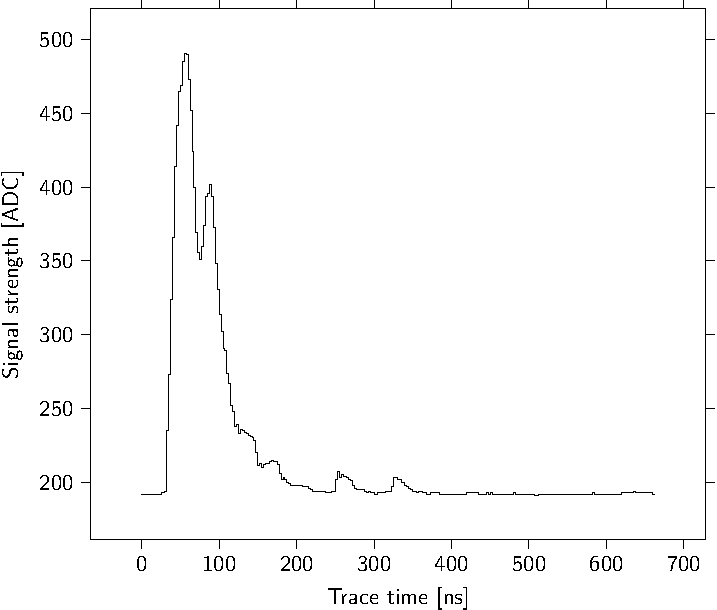
\includegraphics[width=0.7\linewidth]{plots/processing/mean_filter}
    \caption{The same trace as shown in \cref{fig:integral}, except this one is filtered using the Mean Filter. The small peaks and baseline are noticeably smoother.}
    \label{fig:mean_filter}
\end{figure}


\subsection{Trigger pattern}

% Unfortunately not reported correctly for a long time
% Does not specify exact trigger for the event, just highlights which thresholds were triggered
The \hisparc events contain a trigger pattern which indicates which trigger thresholds (including the external trigger) were activated during the trigger window, which of the comparators were triggered, and the presence of slave electronics. A threshold being set to `on' in the trigger threshold pattern does not mean that that threshold actively contributed to the trigger. Take for example a 4-detector station which triggers on 2 high signals. If 2 simultaneous high signals in channels 1 and 2 cause a trigger, and several nano seconds later (still in the trigger window) a high signal appears in channel 3, the high threshold for channel 3 will be marked as active, even though that channel did not actively contribute to the trigger. Therefore, if you wish to know the type of trigger which caused the event it needs to be reconstructed from the event and the station configuration. Moreover, due to a software bug the trigger pattern was stored incorrectly for most data, missing part of the pattern. The trigger pattern is not used in the further analysis.


\subsection{Event rate}

% Definition of event rate
% When it fails to properly represent the actual rate
At each event the average trigger rate (in \si{\hertz}) as measured by the \daq over the last 90 seconds is added to the event. The first few events when starting the \daq will have a too low trigger rate due to the lack of information from the 90 seconds preceding the first triggers. Though not a direct property of the event itself, this provides insight in the proper operation of the detection station.


\subsection{Event data from PC}

The events uploaded for the station to the datastore contain the traces and timestamp and the above described observables, i.e. baselines, pulse heights, pulse integrals, number of peaks, baseline standard deviations, and trigger pattern. The data is stored in a hierarchy which organizes the station data per cluster. Data for each station consist of cosmic ray event data, observed weather data, configurations for both the cosmic-ray and weather hardware and software, errors reported by the software, and since 2016 the single rates and \gps signal strengths are also stored.


\section{Offline processing for the Event Summary Data}

% Daily data processing
The datastore in constantly recieving new data and storing it in the raw datastore. Every morning, several hours after \utc midnight, all new data is processed to generate the Event Summary Data (\esd). Several hours after midnight is used because some stations may be slow in uploading data, this allows extra time to let all events from the previous day come in, and still be finished with processing before the day begins. The event processing also looks for older dates with new events, not just yesterday. Stations have a local buffer in case they are temporarily unable to upload data. There have been cases where a station had several months worth of data locally which was all uploaded once the internet connection was reestablished. By keeping track of modification dates to the raw data files, where data is separated into files per date, it is easy to find dates with new data. The processing applies the event processing module from \sapphire to the data. The following section describe exactly what this involves.


\subsection{Sorting and cleaning}

The first step is the sorting of the events by timestamp, since events are not always uploaded in the correct order. Next, duplicate events are removed. Duplicate events can occur when a station uploading a batch of events to the datastore takes to long and \python reports a timeout, while Windows continues to upload in the background. The \python program will try to upload the data again because it believes the upload failed.


\subsection{Number of particles}

% Fit MPV in pulse integral histogram
% Not yet corrected for inclination
% Assumes leptonic signal
The size of the signals is a measure for the number of particles which passed though the detector. The pulse integral will be used for this since it also accounts for particles which arrive separately in time. Moreover, as shown in \cref{sub:pmt_linearity} the integral is less hindered by saturation of the \adcs. In order to relate the pulse integral to a number of particles the signal strength for a single particle needs to be determined. This is done separately for each detector, since each may be calibrated differently. To determine the signal for a single particle pulse integral data from multiple events is required. As shown in \cref{fig:ph_histogram_contrib} the pulse height histogram is a combination of contributions by a different number of particles and gamma's, the same is true for the pulse integral. By taking a day's worth of events the peak, which is Most Probable Value (\mpv) for a single particle, becomes apparent. By fitting this value a good estimate for the signal of a single particle is achieved. The pulse integral is divided by the fitted \mpv. This number is a first rough estimate for the number of particles. Corrections for the shower angle and \pmt saturation still need to be applied, but those are performed later.

[figure of pulse integral histogram with fitted MPV]


\subsection{Trigger time}
\label{ssec:trigger_time}

% Reconstruct trigger time, may fail for filtered traces
% Used to relate events from different stations
For each event a \gps timestamp is recorded at the moment the trigger conditions are met. Unfortunately, no data is included which connects the \gps timestamp to a specific sample of the traces. This is needed to relate traces from different events and stations. In order to find the sample in the traces to which the \gps timestamp belongs the trigger has to be reconstructed from the trace. Since the trigger conditions are known from the configuration setting this simply requires applying the trigger logic to the traces. The algorithm examines each trace and looks if and when it crosses the low and high thresholds. Then it determines which trigger conditions are first met and at what point in the traces. For a 2-detector station this is simply the second channel that crosses the low threshold. For a 4-detector station either the second high or third low signal, which ever is first. The trigger time is stored relative to the start of the trace. The \hisparc electronics trigger on the raw traces which the \adcs read out, if the Mean Filter is active in the \daq the traces are filtered before they are transmitted to the datastore. This filter sometimes smoothes trace such that signals that actually (raw) crossed a threshold no longer do so in the filtered trace. In some rare cases this causes the wrong moment to be reconstructed or even makes it impossible to reconstruct the trigger. However, this is only the case where low signals or slow rising signals were part of the trigger.

\begin{figure}
    \centering
    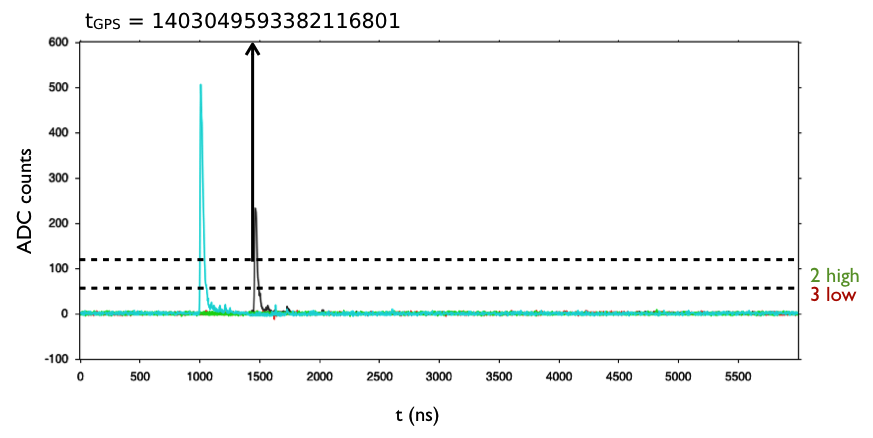
\includegraphics[width=0.7\linewidth]{plots/processing/trigger_time.png}
    \caption{The reconstruction of the trigger time within a trace. For this 4-detector station event the trigger was caused by 2 high signals.}
    \label{fig:trigger_time}
\end{figure}


\subsection{Arrival times}

% Arrival times in individual detectors
The arrival time of particles in each individual detector ($t_i$) is used for direction  reconstruction. The arrival time is defined at the start of the first pulse in a detector, as illustrated in \cref{fig:arrival_time}. For the arrival time the trace signal has to be \SI{20}{\adc} above the baseline to be counted. Like the trigger time the stored arrival time is relative to the start of the trace. Using the \gps timestamp and trigger time these arrival times can be converted to \gps time using $t_{i,\gps} = t_{\gps} - t_{trigger} + t_i$. The arrival times may still be subject to offsets when they need to be related to arrival times in other detectors or stations.

\begin{figure}
    \centering
    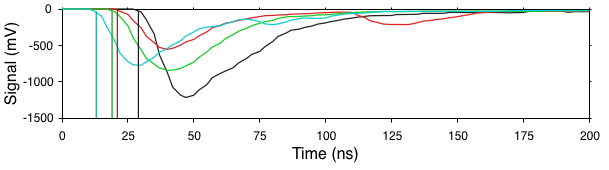
\includegraphics[width=0.7\linewidth]{plots/processing/arrival_time.png}
    \caption{The reconstruction of the arrival time within traces.}
    \label{fig:arrival_time}
\end{figure}


\subsection{Detector offsets}
\label{sec:process_detector_offsets}

% Offsets between detectors in same station
Time offsets are observed between detectors in the same station, as reported in \cref{sec:detector-offsets}. These need to be corrected for to be able to relate the detector arrival times within a station. A single day of data is enough to accurately determine these offsets for the detectors within a station. A four-detector station in the star-layout has approximately \num{60000} triggers per day. A pair of detectors in the outer triangle have approximately \num{12000} triggers in common while a pair which includes the center detector is in approximately \num{14000} triggers. Following from \cref{ssec:efficiency_triggering}, approximately \num{3000} of these triggers per pair are background. Most of the background is easily removed by constraining the maximum allowed time difference between the detectors. Limitting the maximum time difference to the time it would take light to go from one detector to the other, typically \SI{33}{\ns}, removes most background events, leaving only approximately \num{250} background triggers. A small percentage real showers will also be removed, but in those cases the time difference is larger than expected due to shower front thickness and detector transport time effects. Those events do not contribute much to an accurate offset. The timing offset represents what the arrival time difference would be if the detectors were simultaneously hit. This means that the determined offset must also be corrected for the altitude difference between the detectors. The altitude difference causes the detector positioned lower to have later arrival times. For most stations this is irrelevant as the detectors are at the same altitude, but there are some exceptions.

[illustration, show mirror symmetry and altitude effect, offset should correct for difference in case of ` hit]

% Determining the offset, the procedure
First the best detector reference is determined by determining which detector participated in most events with any of the other detectors. In case of 4-detector stations detector 2 will often be this station since it is closest to all other detectors. In case of a 2-detector station detector 2 is always used. After offsets have been determined detector 2 is made the reference by setting its offset to \SI{0}{\ns}. Ideally all offsets are \SI{0}{\ns}, but this is not the case. The distribution off detector timing offsets for all \hisparc stations was shown in \cref{sec:detector-offsets}. The determined offsets must be subtracted from arrival times to get the corrected arrival times.


\subsection{Coincidences}

% Coincidences between multiple stations
After processing data from individual stations their data is combined. First the processed events from all stations of a day are sorted (by timestamp) into a long list. Then coincidences are searched for. A coincidence is a group of least two events for which the \gps timestamps are within \SI{10000}{\ns}, which indicates they are likely from the same air shower. Of course unrelated simultaneous air showers do occur. However, at this stage no further selection is performed other than looking for groups of events which fall within the time window. Events can be present in multiple coincidences as long as a coincidence is not a subset of another coincidence. The coincidences can be used to easily find events from multiple stations caused by the same air shower. In \cref{fig:distance_v_coincidence_rate} the resulting number of coincidences between pairs is seen. For higher order coincidences not only the distances but also the configurations become very important.


\subsection{Station offsets}

% Offsets between stations that are often in coincidence
Finally the timing offset between stations is determined. More than a single day of data is required for this, as reported in \cref{ssec:compensating_gps_offset}. The amount of time required to determine an accurate station offset depends on the coincidence rate between the stations, from \cref{sec:detection-multiple-stations} follows the coincidence rate between stations as a function of their distance. However, as shown in \cref{fig:distance_v_width_sim} the width of the time difference distribution increases with distance between the stations. This is an effect of inclined showers and shower front curvature. With enough coincidences these effects average out and a good offset can be determined. So the distance between stations determines the number of days that will be used for the station offset. Changing \hisparc electronics or the \gps (location or hardware) can change the station offset, such days are therefore excluded and used as boundaries for day ranges. For all station pairs in the \hisparc network with separations less than \SI{1}{\kilo\meter} the offset will be determined. For each event in the coincidences the detector arrival time with the first signal, corrected for detector offsets, is taken to be the arrival time for that station.

% Importance of the offset for stations separated by large distance
When the distance between stations is very large, the expected \gps offsets, of up to \SI{100}{\ns}, become less important as they have less effect on the direction reconstruction. For example, a station pair with a distance of \SI{1}{\kilo\meter} is hit by a flat shower front with an azimuth parallel to the line connecting the two stations and an actual zenith angle of \SI{22.5}{\degree}, an offset of \SI{100}{\ns} between the stations would in this case change the reconstructed zenith by less than \SI{2}{\degree}.

% Explain solution for difficult to determine offsets for distant pairs by using other stations
In some cases pairs of stations are separated by a large distance but have other stations between them that are closer to both. For instance stations 505 and 509 are separated by \SI{580}{\meter}. There are many stations between them which are closer to both, for example station 501 is separated less than \SI{350}{\meter} from both. There are far more coincidences between the pairs 501-505 and 501-509 than 505-509. In this case, using 501 as a stepping stone reduces the time window required to determine an offset between 505-509, and increases the accuracy of the offset. However, in the event that 501 is malfunctioning it may be better to skip it as intermediary.

% Explain best reference/shortest path/accurate offsets algorithm
At some point in a reconstruction one station has to be appointed the reference station. The timing of that station will be considered as correct. In order to minimize the calibration errors the station which has the lowest offset error to all other stations in the coincidence has to be found. This includes offsets via other stations which can increase the accuracy. To determine this the Floyd-Warshall algorithm \cite{floyd1962algorithm} is used to find all the shortest paths between all stations in the coincidence. Here the path lengths between nodes are the square of the error on the offset (i.e. $\sigma^2$) between the station pairs. So the path from station $i$ to station $j$ via $k$ would be $\sigma_{i,j}^2 = \sigma_{i,k}^2 + \sigma_{k,j}^2$. The station with the lowest overall error, i.e. sum of path lengths to all other stations, is used as reference. The paths resulting from the algorithm are reconstructed to calculate the resulting offsets and errors. Note that even stations not part of a coincidence can be used as intermediate steps, but one of the stations in the coincidence has to be the reference.

\begin{figure}
    \centering
    \tikzsetnextfilename{externalized-shortest_path}
 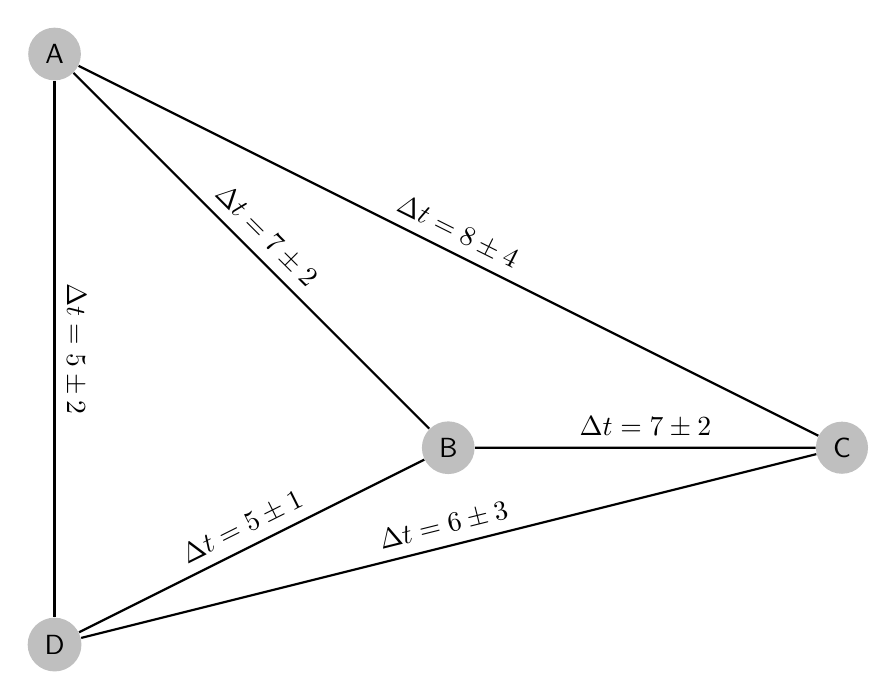
\begin{tikzpicture}
  [scale=2.5,
   font=\sffamily,
   vertex/.style={circle, fill=black!25},
   selected/.style={vertex, fill=red!24},
   edge/.style={draw, thick, -},]
  % Draw the network
  % First we draw the vertices
  \foreach \pos / \name in {{(0,3)/A}, {(2,1)/B}, {(4,1)/C}, {(0,0)/D}}
      \node[vertex] (\name) at \pos {\name};
  % Connect vertices with edges and draw weights
  \foreach \source / \dest / \offset / \error in {
        A/B/7/2,
        A/C/8/4, B/C/7/2,
        A/D/5/2, B/D/5/1, C/D/6/3}
      \path[edge] (\source) -- node[midway, above, sloped, align=left] {
        $\Delta t = \SI{\offset\pm\error}{\ns}$} (\dest);
\end{tikzpicture}

    \caption{Example of determination of best reference and shortest path. [todo highlight shortest paths and reference station]}
    \label{fig:shortest_path}
\end{figure}


\section{Data quality criteria}
\label{sec:data_quality_criteria}

Even if a station has recorded data that does not immediately mean that the data is good and ready to be plugged into the reconstructions. The \gps configuration may have been bad causing inaccurate timestamps, or one of the \pmts may have been oscillating causing bad data in one channel. In this section the criteria for defining good data are discussed. The data that will be used in the analysis will be filtered based on these criteria so that only good data remains.


\subsection{Exclude entire day}

% Exclude station: bad GPS, change of configuration (gps/electronics/voltages)
All data for a station for a day is excluded if something was changed in the configuration of that station. Specifically if the \gps position is altered, different electronics are connected, or the \pmt voltages are changed. If the \gps position changes this can indicate that the station is moved or that a different \gps antenna is connected. All these changes can affect the timing offsets of the station and detectors. A change in the electronics and voltages can also affect the \mpv value of each detector. The offsets and \mpv are determined daily using (multiple) full days as input. Changes to the station which affect these calibration values can cause the fits to be based on mixed datasets. Therefore, those days are excluded from the analysis.

% Exclude detector: bad MPV, bad detector offset
Data from malfunctioning or improperly configured detectors must also be excluded. When determining the particle density in a station only particles and detection area of the working detectors must be counted. If in a 4-detector station one or two detectors are malfunctioning the other two can still trigger on showers. In some cases a malfunctioning detector can cause false signals which will contribute to the triggering of the station. An offline trigger can be used to determine if the station would also have triggered if only the signals of the working detectors are considered. The particle counts and detection area of the bad detectors are excluded when calculating the particle density in the station. In the analysis a bad detector can be recognized by a failed \mpv fit, which means that the derrived particle counts are set to an error value. The arrival times of a detector can not be used if the detector offset was not succefully determined. This could be caused by a small light leak in a detector which skews the arrival times.


\subsection{Specific bad events}

% Exclude entire event: bad t_trigger, trigger on n particles, ...
If trigger time reconstruction fails the event can not be properly placed in absolute \gps timing and can therefore not participate in coincidences. There are two known causes for a failed trigger reconstruction. Either the incorrect trigger configuration is used in the reconstruction or the trace signals are below the thresholds because the mean filter was active. There are some cases in which an updated configuration was not sent to the datastore after it was changed. In case of the filter being the cause the event is likely excluded due to the low signals. After the \mpv for each detector has been determined a new trigger can be defined based on the number of particles in the detector. Using the \mpv and pulse integral the number of particles is estimated more accurately than when using the pulse height, which was used in the trigger on the station. By triggering on the calibrated pulse integral a more consistent trigger is achieved.

% Exclude specific detector: bad baseline (i.e. no n, t)
In some cases the trace of a single detector in an event contains anomalous signals. This can be due to hitches in the \pmt, or due to the event being in the tail of a previous event/strong signal. These cases are likely to result in failed baseline reconstructions, which automatically exclude the detectors from participating in reconstructions since the signal strength and arrival times will also not be reconstructable.


\subsubsection{Software implementation issues}

% Problems in the software which causes some reconstructions to fail
% Acceptable percentage of failed events in case of active filter
As mentioned in the \cref{sec:online} there were some bugs in the software which caused the malformed trigger pattern, traces cut to small, and destructively filtered traces. These were fixed in the \hisparc station software version released at the end of 2015. Most stations still operate on the old version of the software. The cause is that the for some events the trigger time reconstruction fails, which prevents the event from being used in coincidence direction reconstruction. On a daily basis this results in \SI{0.2 \pm 0.1}{\percent} failed trigger time reconstructions. In these events the maximum signal strength will be just above the trigger threshold, and reduced just below it by the filter.
